\documentclass[12pt]{article}

%packages
%\usepackage{latexsym}
\usepackage{graphicx}
\usepackage{wrapfig}
\usepackage{color}
\usepackage{amsmath}
%\usepackage{dsfont}
\usepackage{placeins}
\usepackage{amssymb}
\usepackage{skull}
\usepackage{soul}
%\usepackage{hyperref}
%\usepackage{fancyhdr}

%\fancyhf{} % clear all header and footers
%\renewcommand{\headrulewidth}{0pt} % remove the header rule
%\fancyfoot[LE, LO]{\thepage}


%\usepackage{pstricks,pst-node,pst-tree}

%\usepackage{algpseudocode}
%\usepackage{amsthm}
%\usepackage{hyperref}
%\usepackage{mathrsfs}
%\usepackage{amsfonts}
%\usepackage{bbding}
%\usepackage{listings}
%\usepackage{appendix}
\usepackage[margin=1in]{geometry}
%\geometry{papersize={8.5in,11in},total={6.5in,9in}}
%\usepackage{cancel}
%\usepackage{algorithmic, algorithm}

\newcommand{\qu}[1]{``#1''}
\newcommand{\spc}[1]{\\ \vspace{#1cm}}

\newcounter{probnum}
\setcounter{probnum}{1}
\newcounter{numpts}
\setcounter{numpts}{0}

%create definition to allow local margin changes
\def\changemargin#1#2{\list{}{\rightmargin#2\leftmargin#1}\item[]}
\let\endchangemargin=\endlist 

%allow equations to span multiple pages
\allowdisplaybreaks

%define colors and color typesetting conveniences
\definecolor{gray}{rgb}{0.5,0.5,0.5}
\definecolor{black}{rgb}{0,0,0}
\definecolor{white}{rgb}{1,1,1}
\definecolor{blue}{rgb}{0.5,0.5,1}
\newcommand{\inblue}[1]{\color{blue}#1 \color{black}}
\definecolor{green}{rgb}{0.133,0.545,0.133}
\newcommand{\ingreen}[1]{\color{green}#1 \color{black}}
\definecolor{yellow}{rgb}{1,0.549,0}
\newcommand{\inyellow}[1]{\color{yellow}#1 \color{black}}
\definecolor{red}{rgb}{1,0.133,0.133}
\newcommand{\inred}[1]{\color{red}#1 \color{black}}
\definecolor{purple}{rgb}{0.58,0,0.827}
\newcommand{\inpurple}[1]{\color{purple}#1 \color{black}}
\definecolor{gray}{rgb}{0.5,0.5,0.5}
\newcommand{\ingray}[1]{\color{gray}#1 \color{black}}
\definecolor{backgcode}{rgb}{0.97,0.97,0.8}
\definecolor{Brown}{cmyk}{0,0.81,1,0.60}
\definecolor{OliveGreen}{cmyk}{0.64,0,0.95,0.40}
\definecolor{CadetBlue}{cmyk}{0.62,0.57,0.23,0}

%define new math operators
\DeclareMathOperator*{\argmax}{arg\,max~}
\DeclareMathOperator*{\argmin}{arg\,min~}
\DeclareMathOperator*{\argsup}{arg\,sup~}
\DeclareMathOperator*{\arginf}{arg\,inf~}
\DeclareMathOperator*{\convolution}{\text{\Huge{$\ast$}}}
\newcommand{\infconv}[2]{\convolution^\infty_{#1 = 1} #2}
%true functions

%%%% GENERAL SHORTCUTS

%shortcuts for pure typesetting conveniences
\newcommand{\bv}[1]{\boldsymbol{#1}}

%shortcuts for compound constants
\newcommand{\BetaDistrConst}{\dfrac{\Gamma(\alpha + \beta)}{\Gamma(\alpha)\Gamma(\beta)}}
\newcommand{\NormDistrConst}{\dfrac{1}{\sqrt{2\pi\sigma^2}}}

%shortcuts for conventional symbols
\newcommand{\tsq}{\tau^2}
\newcommand{\tsqh}{\hat{\tau}^2}
\newcommand{\sigsq}{\sigma^2}
\newcommand{\sigsqsq}{\parens{\sigma^2}^2}
\newcommand{\sigsqovern}{\dfrac{\sigsq}{n}}
\newcommand{\tausq}{\tau^2}
\newcommand{\tausqalpha}{\tau^2_\alpha}
\newcommand{\tausqbeta}{\tau^2_\beta}
\newcommand{\tausqsigma}{\tau^2_\sigma}
\newcommand{\betasq}{\beta^2}
\newcommand{\sigsqvec}{\bv{\sigma}^2}
\newcommand{\sigsqhat}{\hat{\sigma}^2}
\newcommand{\sigsqhatmlebayes}{\sigsqhat_{\text{Bayes, MLE}}}
\newcommand{\sigsqhatmle}[1]{\sigsqhat_{#1, \text{MLE}}}
\newcommand{\bSigma}{\bv{\Sigma}}
\newcommand{\bSigmainv}{\bSigma^{-1}}
\newcommand{\thetavec}{\bv{\theta}}
\newcommand{\thetahat}{\hat{\theta}}
\newcommand{\thetahatmle}{\hat{\theta}_{\mathrm{MLE}}}
\newcommand{\thetavechatmle}{\hat{\thetavec}_{\mathrm{MLE}}}
\newcommand{\muhat}{\hat{\mu}}
\newcommand{\musq}{\mu^2}
\newcommand{\muvec}{\bv{\mu}}
\newcommand{\muhatmle}{\muhat_{\text{MLE}}}
\newcommand{\lambdahat}{\hat{\lambda}}
\newcommand{\lambdahatmle}{\lambdahat_{\text{MLE}}}
\newcommand{\etavec}{\bv{\eta}}
\newcommand{\alphavec}{\bv{\alpha}}
\newcommand{\minimaxdec}{\delta^*_{\mathrm{mm}}}
\newcommand{\ybar}{\bar{y}}
\newcommand{\xbar}{\bar{x}}
\newcommand{\Xbar}{\bar{X}}
\newcommand{\iid}{~{\buildrel iid \over \sim}~}
\newcommand{\inddist}{~{\buildrel ind \over \sim}~}
\newcommand{\approxdist}{~{\buildrel approx \over \sim}~}
\newcommand{\equalsindist}{~{\buildrel d \over =}~}
\newcommand{\loglik}[1]{\ell\parens{#1}}
\newcommand{\thetahatkminone}{\thetahat^{(k-1)}}
\newcommand{\thetahatkplusone}{\thetahat^{(k+1)}}
\newcommand{\thetahatk}{\thetahat^{(k)}}
\newcommand{\half}{\frac{1}{2}}
\newcommand{\third}{\frac{1}{3}}
\newcommand{\twothirds}{\frac{2}{3}}
\newcommand{\fourth}{\frac{1}{4}}
\newcommand{\fifth}{\frac{1}{5}}
\newcommand{\sixth}{\frac{1}{6}}

%shortcuts for vector and matrix notation
\newcommand{\A}{\bv{A}}
\newcommand{\At}{\A^T}
\newcommand{\Ainv}{\inverse{\A}}
\newcommand{\B}{\bv{B}}
\newcommand{\K}{\bv{K}}
\newcommand{\Kt}{\K^T}
\newcommand{\Kinv}{\inverse{K}}
\newcommand{\Kinvt}{(\Kinv)^T}
\newcommand{\M}{\bv{M}}
\newcommand{\Bt}{\B^T}
\newcommand{\Q}{\bv{Q}}
\newcommand{\Qt}{\Q^T}
\newcommand{\R}{\bv{R}}
\newcommand{\Rt}{\R^T}
\newcommand{\Z}{\bv{Z}}
\newcommand{\X}{\bv{X}}
\newcommand{\Xsub}{\X_{\text{(sub)}}}
\newcommand{\Xsubadj}{\X_{\text{(sub,adj)}}}
\newcommand{\I}{\bv{I}}
\newcommand{\Y}{\bv{Y}}
\newcommand{\sigsqI}{\sigsq\I}
\renewcommand{\P}{\bv{P}}
\newcommand{\Psub}{\P_{\text{(sub)}}}
\newcommand{\Pt}{\P^T}
\newcommand{\Pii}{P_{ii}}
\newcommand{\Pij}{P_{ij}}
\newcommand{\IminP}{(\I-\P)}
\newcommand{\Xt}{\bv{X}^T}
\newcommand{\XtX}{\Xt\X}
\newcommand{\XtXinv}{\parens{\Xt\X}^{-1}}
\newcommand{\XtXinvXt}{\XtXinv\Xt}
\newcommand{\XXtXinvXt}{\X\XtXinvXt}
\newcommand{\x}{\bv{x}}
\newcommand{\onevec}{\bv{1}}
\newcommand{\oneton}{1, \ldots, n}
\newcommand{\yoneton}{y_1, \ldots, y_n}
\newcommand{\yonetonorder}{y_{(1)}, \ldots, y_{(n)}}
\newcommand{\Yoneton}{Y_1, \ldots, Y_n}
\newcommand{\iinoneton}{i \in \braces{\oneton}}
\newcommand{\onetom}{1, \ldots, m}
\newcommand{\jinonetom}{j \in \braces{\onetom}}
\newcommand{\xoneton}{x_1, \ldots, x_n}
\newcommand{\Xoneton}{X_1, \ldots, X_n}
\newcommand{\xt}{\x^T}
\newcommand{\y}{\bv{y}}
\newcommand{\yt}{\y^T}
\renewcommand{\c}{\bv{c}}
\newcommand{\ct}{\c^T}
\newcommand{\tstar}{\bv{t}^*}
\renewcommand{\u}{\bv{u}}
\renewcommand{\v}{\bv{v}}
\renewcommand{\a}{\bv{a}}
\newcommand{\s}{\bv{s}}
\newcommand{\yadj}{\y_{\text{(adj)}}}
\newcommand{\xjadj}{\x_{j\text{(adj)}}}
\newcommand{\xjadjM}{\x_{j \perp M}}
\newcommand{\yhat}{\hat{\y}}
\newcommand{\yhatsub}{\yhat_{\text{(sub)}}}
\newcommand{\yhatstar}{\yhat^*}
\newcommand{\yhatstarnew}{\yhatstar_{\text{new}}}
\newcommand{\z}{\bv{z}}
\newcommand{\zt}{\z^T}
\newcommand{\bb}{\bv{b}}
\newcommand{\bbt}{\bb^T}
\newcommand{\bbeta}{\bv{\beta}}
\newcommand{\beps}{\bv{\epsilon}}
\newcommand{\bepst}{\beps^T}
\newcommand{\e}{\bv{e}}
\newcommand{\Mofy}{\M(\y)}
\newcommand{\KofAlpha}{K(\alpha)}
\newcommand{\ellset}{\mathcal{L}}
\newcommand{\oneminalph}{1-\alpha}
\newcommand{\SSE}{\text{SSE}}
\newcommand{\SSEsub}{\text{SSE}_{\text{(sub)}}}
\newcommand{\MSE}{\text{MSE}}
\newcommand{\RMSE}{\text{RMSE}}
\newcommand{\SSR}{\text{SSR}}
\newcommand{\SST}{\text{SST}}
\newcommand{\JSest}{\delta_{\text{JS}}(\x)}
\newcommand{\Bayesest}{\delta_{\text{Bayes}}(\x)}
\newcommand{\EmpBayesest}{\delta_{\text{EmpBayes}}(\x)}
\newcommand{\BLUPest}{\delta_{\text{BLUP}}}
\newcommand{\MLEest}[1]{\hat{#1}_{\text{MLE}}}

%shortcuts for Linear Algebra stuff (i.e. vectors and matrices)
\newcommand{\twovec}[2]{\bracks{\begin{array}{c} #1 \\ #2 \end{array}}}
\newcommand{\threevec}[3]{\bracks{\begin{array}{c} #1 \\ #2 \\ #3 \end{array}}}
\newcommand{\fivevec}[5]{\bracks{\begin{array}{c} #1 \\ #2 \\ #3 \\ #4 \\ #5 \end{array}}}
\newcommand{\twobytwomat}[4]{\bracks{\begin{array}{cc} #1 & #2 \\ #3 & #4 \end{array}}}
\newcommand{\threebytwomat}[6]{\bracks{\begin{array}{cc} #1 & #2 \\ #3 & #4 \\ #5 & #6 \end{array}}}

%shortcuts for conventional compound symbols
\newcommand{\thetainthetas}{\theta \in \Theta}
\newcommand{\reals}{\mathbb{R}}
\newcommand{\complexes}{\mathbb{C}}
\newcommand{\rationals}{\mathbb{Q}}
\newcommand{\integers}{\mathbb{Z}}
\newcommand{\naturals}{\mathbb{N}}
\newcommand{\forallninN}{~~\forall n \in \naturals}
\newcommand{\forallxinN}[1]{~~\forall #1 \in \reals}
\newcommand{\matrixdims}[2]{\in \reals^{\,#1 \times #2}}
\newcommand{\inRn}[1]{\in \reals^{\,#1}}
\newcommand{\mathimplies}{\quad\Rightarrow\quad}
\newcommand{\mathlogicequiv}{\quad\Leftrightarrow\quad}
\newcommand{\eqncomment}[1]{\quad \text{(#1)}}
\newcommand{\limitn}{\lim_{n \rightarrow \infty}}
\newcommand{\limitN}{\lim_{N \rightarrow \infty}}
\newcommand{\limitd}{\lim_{d \rightarrow \infty}}
\newcommand{\limitt}{\lim_{t \rightarrow \infty}}
\newcommand{\limitsupn}{\limsup_{n \rightarrow \infty}~}
\newcommand{\limitinfn}{\liminf_{n \rightarrow \infty}~}
\newcommand{\limitk}{\lim_{k \rightarrow \infty}}
\newcommand{\limsupn}{\limsup_{n \rightarrow \infty}}
\newcommand{\limsupk}{\limsup_{k \rightarrow \infty}}
\newcommand{\floor}[1]{\left\lfloor #1 \right\rfloor}
\newcommand{\ceil}[1]{\left\lceil #1 \right\rceil}

%shortcuts for environments
\newcommand{\beqn}{\vspace{-0.25cm}\begin{eqnarray*}}
\newcommand{\eeqn}{\end{eqnarray*}}
\newcommand{\bneqn}{\vspace{-0.25cm}\begin{eqnarray}}
\newcommand{\eneqn}{\end{eqnarray}}
\newcommand{\benum}{\begin{enumerate}}
\newcommand{\eenum}{\end{enumerate}}

%shortcuts for mini environments
\newcommand{\parens}[1]{\left(#1\right)}
\newcommand{\squared}[1]{\parens{#1}^2}
\newcommand{\tothepow}[2]{\parens{#1}^{#2}}
\newcommand{\prob}[1]{\mathbb{P}\parens{#1}}
\newcommand{\littleo}[1]{o\parens{#1}}
\newcommand{\bigo}[1]{O\parens{#1}}
\newcommand{\Lp}[1]{\mathbb{L}^{#1}}
\renewcommand{\arcsin}[1]{\text{arcsin}\parens{#1}}
\newcommand{\prodonen}[2]{\bracks{\prod_{#1=1}^n #2}}
\newcommand{\mysum}[4]{\sum_{#1=#2}^{#3} #4}
\newcommand{\sumonen}[2]{\sum_{#1=1}^n #2}
\newcommand{\infsum}[2]{\sum_{#1=1}^\infty #2}
\newcommand{\infprod}[2]{\prod_{#1=1}^\infty #2}
\newcommand{\infunion}[2]{\bigcup_{#1=1}^\infty #2}
\newcommand{\infinter}[2]{\bigcap_{#1=1}^\infty #2}
\newcommand{\infintegral}[2]{\int^\infty_{-\infty} #2 ~\text{d}#1}
\newcommand{\supthetas}[1]{\sup_{\thetainthetas}\braces{#1}}
\newcommand{\bracks}[1]{\left[#1\right]}
\newcommand{\braces}[1]{\left\{#1\right\}}
\newcommand{\set}[1]{\left\{#1\right\}}
\newcommand{\abss}[1]{\left|#1\right|}
\newcommand{\norm}[1]{\left|\left|#1\right|\right|}
\newcommand{\normsq}[1]{\norm{#1}^2}
\newcommand{\inverse}[1]{\parens{#1}^{-1}}
\newcommand{\rowof}[2]{\parens{#1}_{#2\cdot}}

%shortcuts for functionals
\newcommand{\realcomp}[1]{\text{Re}\bracks{#1}}
\newcommand{\imagcomp}[1]{\text{Im}\bracks{#1}}
\newcommand{\range}[1]{\text{range}\bracks{#1}}
\newcommand{\colsp}[1]{\text{colsp}\bracks{#1}}
\newcommand{\rowsp}[1]{\text{rowsp}\bracks{#1}}
\newcommand{\tr}[1]{\text{tr}\bracks{#1}}
\newcommand{\rank}[1]{\text{rank}\bracks{#1}}
\newcommand{\proj}[2]{\text{Proj}_{#1}\bracks{#2}}
\newcommand{\projcolspX}[1]{\text{Proj}_{\colsp{\X}}\bracks{#1}}
\newcommand{\median}[1]{\text{median}\bracks{#1}}
\newcommand{\mean}[1]{\text{mean}\bracks{#1}}
\newcommand{\dime}[1]{\text{dim}\bracks{#1}}
\renewcommand{\det}[1]{\text{det}\bracks{#1}}
\newcommand{\expe}[1]{\mathbb{E}\bracks{#1}}
\newcommand{\expeabs}[1]{\expe{\abss{#1}}}
\newcommand{\expesub}[2]{\mathbb{E}_{#1}\bracks{#2}}
\newcommand{\indic}[1]{\mathds{1}_{#1}}
\newcommand{\var}[1]{\mathbb{V}\text{ar}\bracks{#1}}
\newcommand{\sd}[1]{\mathbb{S}\text{D}\bracks{#1}}
\newcommand{\cov}[2]{\text{Cov}\bracks{#1, #2}}
\newcommand{\corr}[2]{\text{Corr}\bracks{#1, #2}}
\newcommand{\se}[1]{\text{SE}\bracks{#1}}
\newcommand{\seest}[1]{\hat{\text{SE}}\bracks{#1}}
\newcommand{\bias}[1]{\text{Bias}\bracks{#1}}
\newcommand{\partialop}[2]{\dfrac{\partial}{\partial #1}\bracks{#2}}
\newcommand{\secpartialop}[2]{\dfrac{\partial^2}{\partial #1^2}\bracks{#2}}
\newcommand{\mixpartialop}[3]{\dfrac{\partial^2}{\partial #1 \partial #2}\bracks{#3}}

%shortcuts for functions
\renewcommand{\exp}[1]{\mathrm{exp}\parens{#1}}
\renewcommand{\cos}[1]{\text{cos}\parens{#1}}
\renewcommand{\sin}[1]{\text{sin}\parens{#1}}
\newcommand{\sign}[1]{\text{sign}\parens{#1}}
\newcommand{\are}[1]{\mathrm{ARE}\parens{#1}}
\newcommand{\natlog}[1]{\ln\parens{#1}}
\newcommand{\oneover}[1]{\frac{1}{#1}}
\newcommand{\overtwo}[1]{\frac{#1}{2}}
\newcommand{\overn}[1]{\frac{#1}{n}}
\newcommand{\oneoversqrt}[1]{\oneover{\sqrt{#1}}}
\newcommand{\sqd}[1]{\parens{#1}^2}
\newcommand{\loss}[1]{\ell\parens{\theta, #1}}
\newcommand{\losstwo}[2]{\ell\parens{#1, #2}}
\newcommand{\cf}{\phi(t)}

%English language specific shortcuts
\newcommand{\ie}{\textit{i.e.} }
\newcommand{\AKA}{\textit{AKA} }
\renewcommand{\iff}{\textit{iff}}
\newcommand{\eg}{\textit{e.g.} }
\renewcommand{\st}{\textit{s.t.} }
\newcommand{\wrt}{\textit{w.r.t.} }
\newcommand{\mathst}{~~\text{\st}~~}
\newcommand{\mathand}{~~\text{and}~~}
\newcommand{\ala}{\textit{a la} }
\newcommand{\ppp}{posterior predictive p-value}
\newcommand{\dd}{dataset-to-dataset}

%shortcuts for distribution titles
\newcommand{\logistic}[2]{\mathrm{Logistic}\parens{#1,\,#2}}
\newcommand{\bernoulli}[1]{\mathrm{Bernoulli}\parens{#1}}
\newcommand{\betanot}[2]{\mathrm{Beta}\parens{#1,\,#2}}
\newcommand{\stdbetanot}{\betanot{\alpha}{\beta}}
\newcommand{\multnormnot}[3]{\mathcal{N}_{#1}\parens{#2,\,#3}}
\newcommand{\normnot}[2]{\mathcal{N}\parens{#1,\,#2}}
\newcommand{\classicnormnot}{\normnot{\mu}{\sigsq}}
\newcommand{\stdnormnot}{\normnot{0}{1}}
\newcommand{\uniform}[2]{\mathrm{U}\parens{#1,\,#2}}
\newcommand{\stduniform}{\uniform{0}{1}}
\newcommand{\exponential}[1]{\mathrm{Exp}\parens{#1}}
\newcommand{\gammadist}[2]{\mathrm{Gamma}\parens{#1, #2}}
\newcommand{\poisson}[1]{\mathrm{Poisson}\parens{#1}}
\newcommand{\binomial}[2]{\mathrm{Binomial}\parens{#1,\,#2}}
\newcommand{\rayleigh}[1]{\mathrm{Rayleigh}\parens{#1}}
\newcommand{\multinomial}[2]{\mathrm{Multinomial}\parens{#1,\,#2}}
\newcommand{\gammanot}[2]{\mathrm{Gamma}\parens{#1,\,#2}}
\newcommand{\cauchynot}[2]{\text{Cauchy}\parens{#1,\,#2}}
\newcommand{\invchisqnot}[1]{\text{Inv}\chisq{#1}}
\newcommand{\invscaledchisqnot}[2]{\text{ScaledInv}\ncchisq{#1}{#2}}
\newcommand{\invgammanot}[2]{\text{InvGamma}\parens{#1,\,#2}}
\newcommand{\chisq}[1]{\chi^2_{#1}}
\newcommand{\ncchisq}[2]{\chi^2_{#1}\parens{#2}}
\newcommand{\ncF}[3]{F_{#1,#2}\parens{#3}}

%shortcuts for PDF's of common distributions
\newcommand{\logisticpdf}[3]{\oneover{#3}\dfrac{\exp{-\dfrac{#1 - #2}{#3}}}{\parens{1+\exp{-\dfrac{#1 - #2}{#3}}}^2}}
\newcommand{\betapdf}[3]{\dfrac{\Gamma(#2 + #3)}{\Gamma(#2)\Gamma(#3)}#1^{#2-1} (1-#1)^{#3-1}}
\newcommand{\normpdf}[3]{\frac{1}{\sqrt{2\pi#3}}\exp{-\frac{1}{2#3}(#1 - #2)^2}}
\newcommand{\normpdfvarone}[2]{\dfrac{1}{\sqrt{2\pi}}e^{-\half(#1 - #2)^2}}
\newcommand{\chisqpdf}[2]{\dfrac{1}{2^{#2/2}\Gamma(#2/2)}\; {#1}^{#2/2-1} e^{-#1/2}}
\newcommand{\invchisqpdf}[2]{\dfrac{2^{-\overtwo{#1}}}{\Gamma(#2/2)}\,{#1}^{-\overtwo{#2}-1}  e^{-\oneover{2 #1}}}
\newcommand{\uniformdiscrete}[1]{\mathrm{Uniform}\parens{\braces{#1}}}
\newcommand{\exponentialpdf}[2]{#2\exp{-#2#1}}
\newcommand{\poissonpdf}[2]{\dfrac{e^{-#1} #1^{#2}}{#2!}}
\newcommand{\binomialpdf}[3]{\binom{#2}{#1}#3^{#1}(1-#3)^{#2-#1}}
\newcommand{\rayleighpdf}[2]{\dfrac{#1}{#2^2}\exp{-\dfrac{#1^2}{2 #2^2}}}
\newcommand{\gammapdf}[3]{\dfrac{#3^#2}{\Gamma\parens{#2}}#1^{#2-1}\exp{-#3 #1}}
\newcommand{\cauchypdf}[3]{\oneover{\pi} \dfrac{#3}{\parens{#1-#2}^2 + #3^2}}
\newcommand{\Gammaf}[1]{\Gamma\parens{#1}}

%shortcuts for miscellaneous typesetting conveniences
\newcommand{\notesref}[1]{\marginpar{\color{gray}\tt #1\color{black}}}

%%%% DOMAIN-SPECIFIC SHORTCUTS

%Real analysis related shortcuts
\newcommand{\zeroonecl}{\bracks{0,1}}
\newcommand{\forallepsgrzero}{\forall \epsilon > 0~~}
\newcommand{\lessthaneps}{< \epsilon}
\newcommand{\fraccomp}[1]{\text{frac}\bracks{#1}}

%Bayesian related shortcuts
\newcommand{\yrep}{y^{\text{rep}}}
\newcommand{\yrepisq}{(\yrep_i)^2}
\newcommand{\yrepvec}{\bv{y}^{\text{rep}}}


%Probability shortcuts
\newcommand{\SigField}{\mathcal{F}}
\newcommand{\ProbMap}{\mathcal{P}}
\newcommand{\probtrinity}{\parens{\Omega, \SigField, \ProbMap}}
\newcommand{\convp}{~{\buildrel p \over \rightarrow}~}
\newcommand{\convLp}[1]{~{\buildrel \Lp{#1} \over \rightarrow}~}
\newcommand{\nconvp}{~{\buildrel p \over \nrightarrow}~}
\newcommand{\convae}{~{\buildrel a.e. \over \longrightarrow}~}
\newcommand{\convau}{~{\buildrel a.u. \over \longrightarrow}~}
\newcommand{\nconvau}{~{\buildrel a.u. \over \nrightarrow}~}
\newcommand{\nconvae}{~{\buildrel a.e. \over \nrightarrow}~}
\newcommand{\convd}{~{\buildrel \mathcal{D} \over \rightarrow}~}
\newcommand{\nconvd}{~{\buildrel \mathcal{D} \over \nrightarrow}~}
\newcommand{\withprob}{~~\text{w.p.}~~}
\newcommand{\io}{~~\text{i.o.}}

\newcommand{\Acl}{\bar{A}}
\newcommand{\ENcl}{\bar{E}_N}
\newcommand{\diam}[1]{\text{diam}\parens{#1}}

\newcommand{\taua}{\tau_a}

\newcommand{\myint}[4]{\int_{#2}^{#3} #4 \,\text{d}#1}
\newcommand{\laplacet}[1]{\mathscr{L}\bracks{#1}}
\newcommand{\laplaceinvt}[1]{\mathscr{L}^{-1}\bracks{#1}}
\renewcommand{\min}[1]{\text{min}\braces{#1}}

\newcommand{\Vbar}[1]{\bar{V}\parens{#1}}
\newcommand{\expnegrtau}{\exp{-r\tau}}
\newcommand{\cprob}[2]{\prob{#1~|~#2}}

%%% problem typesetting
\newcommand{\problem}{\vspace{0.2cm} \noindent {\large{\textsf{Problem \arabic{probnum}~}}} \addtocounter{probnum}{1}}
%\newcommand{\easyproblem}{\ingreen{\noindent \textsf{Problem \arabic{probnum}~}} \addtocounter{probnum}{1}}
%\newcommand{\intermediateproblem}{\noindent \inyellow{\textsf{Problem \arabic{probnum}~}} \addtocounter{probnum}{1}}
%\newcommand{\hardproblem}{\inred{\noindent \textsf{Problem \arabic{probnum}~}} \addtocounter{probnum}{1}}
%\newcommand{\extracreditproblem}{\noindent \inpurple{\textsf{Problem \arabic{probnum}~}} \addtocounter{probnum}{1}}

\newcommand{\easysubproblem}{\ingreen{\item}}
\newcommand{\intermediatesubproblem}{\inyellow{\item}}
\newcommand{\hardsubproblem}{\inred{\item}}
\newcommand{\extracreditsubproblem}{\inpurple{\item}}
\renewcommand{\labelenumi}{(\alph{enumi})}
%\newcommand{\subquestionwithpoints}[1]{\addtocounter{numpts}{#1} \item \ingray{[#1 pt]}~~} %  / \arabic{numpts} pts
\newcommand{\subquestionwithpoints}[1]{\addtocounter{numpts}{#1} \item \ingray{[#1 pt / \arabic{numpts} pts]}~~}  

\newtoggle{professormode}
\toggletrue{professormode} %STUDENTS: DELETE or COMMENT this line



\title{MATH 241 Fall 2015 Homework \#10}

\author{Professor Adam Kapelner} %STUDENTS: write your name here

\iftoggle{professormode}{
\date{Due 4PM in my mail slot, Friday, December 4, 2015 \\ \vspace{0.5cm} \small (this document last updated \today ~at \currenttime)}
}

\renewcommand{\abstractname}{Instructions and Philosophy}




\begin{document}
\maketitle

\iftoggle{professormode}{
\begin{abstract}
The path to success in this class is to do many problems. Unlike other courses, exclusively doing reading(s) will not help. Coming to lecture is akin to watching workout videos; thinking about and solving problems on your own is the actual ``working out.''  Feel free to \qu{work out} with others; \textbf{I want you to work on this in groups.}

Reading is still \textit{required}. For this homework set, read about moment generating functions and their properties and read about the central limit theorem.

The problems below are color coded: \ingreen{green} problems are considered \textit{easy} and marked \qu{[easy]}; \inorange{yellow} problems are considered \textit{intermediate} and marked \qu{[harder]}, \inred{red} problems are considered \textit{difficult} and marked \qu{[difficult]} and \inpurple{purple} problems are extra credit. The \textit{easy} problems are intended to be ``giveaways'' if you went to class. Do as much as you can of the others; I expect you to at least attempt the \textit{difficult} problems.

This homework is worth 100 points but the point distribution will not be determined until after the due date. See syllabus for the policy on late homework.

Up to 15 points are given as a bonus if the homework is typed using \LaTeX. Links to instaling \LaTeX~and program for compiling \LaTeX~is found on the syllabus. You are encouraged to use \url{overleaf.com}. If you are handing in homework this way, read the comments in the code; there are two lines to comment out and you should replace my name with yours and write your section. The easiest way to use overleaf is to copy the raw text from hwxx.tex and preamble.tex into two new overleaf tex files with the same name (thanks to Anastassiya and Jasmine of Section A for figuring this out). If you are asked to make drawings, you can take a picture of your handwritten drawing and insert them as figures or leave space using the \qu{$\backslash$vspace} command and draw them in after printing or attach them stapled.

The document is available with spaces for you to write your answers. If not using \LaTeX, print this document and write in your answers. I do not accept homeworks which are \textit{not} on this printout. Keep this first page printed for your records. Write your name and section below (A, B or C). 10 points off if your section is blank or wrong.

\end{abstract}

\thispagestyle{empty}
\vspace{1cm}
NAME: \line(1,0){240} ~~SECTION (A, B or C): \line(1,0){35} \\
\clearpage
}


\iftoggle{professormode}{
\paragraph{Moment Generating Functions} There are a few facts to know for the exam. This is what you are responsible for.\\ \\
} 

\problem{In this problem you will be introduced to mgf's and learn the three facts about them that we will make use of (1) that mgf's can give you moments easily and (2) it is easy to obtain the mgf of convolutions of r.v.'s. (3) r.v.'s with equivalent mgf's have equivalent CDF's, making them identically distributed.}

\begin{enumerate}

\easysubproblem{What is a moment generating function (mgf)? Read about it in the book and answer a few sentences \textit{in English}. }\spc{2}

\easysubproblem{Using the definition of expectation, write out what $\expe{g(X)}$ is for a discrete r.v. $X$. This can be found in the notes from previous lectures. }\spc{2}

\easysubproblem{Using the definition of expectation, write out what $\expe{g(X)}$ is for a continuous r.v. $X$. This can be found in the notes from previous lectures. }\spc{2}

\easysubproblem{For the mgf, what is the $g(X)$ transformation we are interested in finding the expectation of? Write $g(X) = $ something below. }\spc{2}

\easysubproblem{If $X$ is a discrete r.v., write the definition of the mgf, $M_X(t)$. If you use the notation $f(x)$ make sure you indicate what you are referring to. If you use the notation $\expe{\cdot}$, make sure you indicate the mathematical definition of the expectation. }\spc{2}

\easysubproblem{If $X$ is a continuous r.v., write the definition of the mgf, $M_X(t)$. If you use the notation $f(x)$ make sure you indicate what you are referring to. If you use the notation $\expe{\cdot}$, make sure you indicate the mathematical definition of the expectation.  }\spc{2}

\easysubproblem{Using the Taylor series definition of the exponential function, write out the first five terms of what $e^{tX}$ is and then write $+~\ldots$ afterwards.  }\spc{2}

\easysubproblem{Using your answer from part (g), write the first five terms of $\expe{ e^{tX} }$ using the property of expectation being a linear operator (\ie $\expe{X+Y} = \expe{X} + \expe{Y}$ which is valid always) and then write $+ ~\expe{\ldots}$ afterwards.  }\spc{1.5}

\easysubproblem{You have written the first five terms of the infinite series representation of $M_X(t)$, the mgf for a r.v. $X$ in the previous problem. Now find $M'_X(t)$, the derivative of the mgf with respect to $t$, the dummy variable in the $t$ domain and then write $+~ \ldots$ afterwards. Remember, anything that's a function of the r.v. $X$ is a constant when differentiating with respect to $t$.  }\spc{1.5}

\easysubproblem{Find $M'_X(0)$, \ie the derivative of the mgf evaluated at $t=0$. Ignore terms after the ...  }\spc{4}

\easysubproblem{Find $M''_X(t)$, the second derivative of the mgf with respect to $t$ and then write $+ \ldots$ afterwards.  }\spc{2}

\easysubproblem{Find $M''_X(0)$, \ie the second derivative of the mgf evaluated at $t=0$. Ignore terms after the ...  }\spc{2}

\easysubproblem{Find $M'''_X(t)$, the third derivative of the mgf with respect to $t$ and then write $+ \ldots$ afterwards.  }\spc{2}

\easysubproblem{Find $M'''_X(0)$, \ie the third derivative of the mgf evaluated at $t=0$. Ignore terms after the ...  }\spc{2}

\easysubproblem{When evaluating parts (j), (l), (n) at $t=0$, why do you think you're entitled to ignore terms after the ...? Write a sentence \textit{in English}.  }\spc{2}

\easysubproblem{Synthesize your answers to the last 7 parts and explain why the mgf is called the \qu{moment generating} function \textit{in English}.  }\spc{2}

\easysubproblem{Let $X_1$ and $X_2$ be two independent r.v's (not necessarily identically distributed). Show that $M_{X_1+X_2}(t) = M_{X_1}(t)M_{X_2}(t)$.  }\spc{2}

\intermediatesubproblem{Generalize this reasoning and show that for $X_1, X_2, \ldots, X_n$, a series of independent r.v.'s discrete or continuous and $T_n = \sum_{i=1}^n X_i$ that the following is true:

\beqn
M_{T_n}(t) = \prod_{i=1}^n M_{X_i}(t)
\eeqn  }\spc{3}

\hardsubproblem{In (q) and (r), why do we need independence to prove these facts? Write a couple sentences \textit{in English} referencing the lecture where we went over this.  }\spc{3}

\intermediatesubproblem{Let $Y = X + c$ where $X$ is a r.v. either discrete or continuous and $c \in \reals$ is a constant. Let $M_X(t)$ denote the mgf for the r.v. $X$. Find $M_Y(t)$, the mgf for the shifted r.v. $Y$ as a function of $M_X(t)$.  }\spc{5}

\hardsubproblem{Let $Y = aX$ where $X$ is a r.v. either discrete or continuous and $a \in \reals$ is a constant. Let $M_X(t)$ denote the mgf for the r.v. $X$. Find $M_Y(t)$, the mgf for the scaled r.v. $Y$ as a function of $M_X(t)$.  }\spc{2}

\end{enumerate}

\problem{Here, we will be deriving mgf's of some of our brand name r.v.'s and using them to prove cool things about distribution theory.}


\begin{enumerate}
\easysubproblem{Let $X \sim \bernoulli{p}$. Show that $\expe{X^{37}} = p$ using the definition of expectation. I will begin the problem below for you: 

\beqn
\expe{X^{37}} &=& \sum_{x \in \support{X}} x^{37} f(x) = \sum_{x=0}^1 x^{37} p^x (1-p)^{1-x} \\
&=&
\eeqn
}\spc{2}

\intermediatesubproblem{Using the definition of the mgf, find $M_X(t)$, the mgf for a Bernoulli r.v.}\spc{2}


\hardsubproblem{Show that $\expe{X^{37}} = p$ using the mgf and the fact you proved in question 1(o). You may have to use English to explain what you're doing. I do not expect you to take 37 derivatives, but you should take at least two and see the pattern.}\spc{5}


\hardsubproblem{Let $T \sim \binomial{n}{p}$. Find the mgf of $X$ using the definition of the mgf. You will need to invoke the binomial theorem here (see class notes). }\spc{4}


\intermediatesubproblem{Using the fact you proved in 1(r), use mgf's to show that $T = X_1 + \ldots + X_n$ where $T$ is the binomial r.v. from the previous problem and $X_1, \ldots, X_n \iid \bernoulli{p}$. }\spc{3}




\hardsubproblem{Show that the sum of two independent r.v.'s $T_1 \sim \binomial{n_1}{p}$ and $T_2 \sim \binomial{n_2}{p}$ is a new r.v. which itself is a binomial and find its parameters. Does this make sense given what you proved in (e)? }\spc{4}


\easysubproblem{Let $X_1, \ldots, X_r \iid \geometric{p}$. Assume that the mgf for the geometric is:

\beqn
M_{X_i}(t) = \frac{pe^t}{1-(1-p) e^t}
\eeqn

Let $T = X_1 + \ldots + X_r$. We know from our study of discrete r.v.'s that $T \sim \negbin{r}{p}$ which was illustrated conceptually. However, this was never proven. We will prove it here. Using the fact that:

\beqn
M_T(t) = \tothepow{\frac{pe^t}{1-(1-p) e^t}}{r}
\eeqn

for the negative binomial r.v., show that negative binomial r.v.'s are indeed the sum of many $\iid$ geometric r.v.'s using the fact you proved in 1(r). This looks hard but it is marked easy, so I assure you: it is easy! (It is not easy if you do not have mgf's, really really not easy).  }\spc{4}

\intermediatesubproblem{Show that the sum of two independent r.v.'s $T_1 \sim \negbin{r_1}{p}$ and $T_2 \sim \negbin{r_2}{p}$ is itself a negative binomial and find its parameters. This was on a practice midterm. }\spc{7}

\hardsubproblem{Let $X \sim \poisson{\lambda}$ with mgf:

\beqn
M_X(t) = e^{\lambda (e^t - 1)}
\eeqn

Show that the sum of two independent r.v.'s $X_1 \sim \poisson{\lambda_1}$ and $X_2 \sim \poisson{\lambda_2}$ is itself a Poisson r.v. and find its parameter. You don't even need to know what the Poisson is for this question.}\spc{4}

\hardsubproblem{You have shown previously that the mgf for the r.v. $X \sim \binomial{n}{p}$ was $M_X(t) = \tothepow{1-p+pe^t}{n}$. In the previous problem you were given the mgf for the r.v. $X \sim \poisson{\lambda}$ was $M_X(t) = e^{\lambda (e^t - 1)}$. Although we didn't cover it in class, the Poisson distribution is the limit of the Binomial distribution with $n \rightarrow \infty$ and the rate parameter pinned $\lambda = np$. Prove that the Poisson's mgf is this limit of the Binomial's mgf. Really not hard: just some algebraic manipulations. Let $p = \lambda / n$.}\spc{4}

\intermediatesubproblem{We proved in class that if $Z \sim \stdnormnot$ then $M_Z(t) = e^{t^2/2}$. We also showed that if $X = \sigma Z + \mu$, then $X \sim \normnot{\mu}{\sigsq}$. Show that the mgf of $X$ is $M_X(t) = e^{\mu t + \sigsq t^2 /2}$ using what you learned in quesiton 1 and the class notes.  }\spc{4}

\hardsubproblem{Let $X_1, X_2, \ldots, X_n$ be a sequence of independent normal random variables where $X_1$ has mean $\mu_1$ and variance $\sigsq_1$ and $X_2$ has mean $\mu_2$ and variance $\sigsq_2$, etc. Show that $X_1 + X_2 + \ldots + X_n$ is normally distributed and find its parameters.  }\spc{6}

\extracreditsubproblem{Let $X \sim \exponential{\lambda}$ with mgf:

\beqn
M_X(t) = \frac{\lambda}{\lambda - t}
\eeqn

Demonstrate that the sum of $X_1, \ldots, X_n \iid \exponential{\lambda}$ is an Erlang r.v. with parameters $n$ and $\lambda$, the continuous analogue of the Negative Binomial r.v.  (You will need to look up the mgf of the Erlang distribution). Do on a separate piece of paper.}

\extracreditsubproblem{The standard Cauchy distribution has center 0 and scale parameter 1 and its PDF is:

\beqn
f(x) = \oneover{\pi(1+x^2)}
\eeqn

The Cauchy distribution is a classic example of a pathological r.v. You'll see why. The standard Cauchy r.v. is actually the ratio of two independent standard normal r.v.'s: if $X \sim \stdnormnot$ and $Y \sim \stdnormnot$ then $X/Y$ has the PDF above.

Prove that the mgf for a standard Cauchy r.v. does not exist. This is really not hard but it looks menacing. Do on a separate piece of paper. }


\end{enumerate}

\iftoggle{professormode}{
\paragraph{Central Limit Theorem} We will introduce it here and provide some illustrations.\\ \\
} 

\problem{We will now prove the \qu{Central Limit Theorem} (the CLT), the crown jewel of a college-level course on probability. I will not ask you to prove it on the exam, but I may ask you general questions about the proof. The best thing to do then, is to prove it yourself in which case you'll be prepared for basic questions. You will not be asked to do anything other than to critically read and synthesize the lecture notes.}

\begin{enumerate}
\intermediatesubproblem{We start by looking at r.v.'s $X_1, X_2, \ldots, X_n$. What are the assumptions on these r.v.'s? There are three.  }\spc{4}

\easysubproblem{We started our proof examining $\Xbar_n$. What is $\expe{\Xbar_n}$?  }\spc{2}

\easysubproblem{What is $\se{\Xbar_n}$. I'm marking this easy because you've done it before and it's in the notes.  }\spc{2}

\easysubproblem{Below is its standardized form.

\beqn
C_n = \frac{\Xbar_n - \mu}{\frac{\sigma}{\sqrt{n}}}
\eeqn

If it's \qu{standardized,} what is the mean and standard error of $C_n$?  }\spc{2}

\easysubproblem{Show that $C_n = \frac{Z_1}{\sqrt{n}} + \frac{Z_2}{\sqrt{n}} + \ldots + \frac{Z_n}{\sqrt{n}}$.  }\spc{3}

\intermediatesubproblem{Find the first five terms of $e^{tZ}$ using the Taylor Series. You can put $+~\ldots$ after the five terms. This is the same thing you did in 1(g).  }\spc{4}

\easysubproblem{Find the first five terms of $M_Z(t)$, the mgf of all the $Z_i$'s (which are $\iid$). This just means take the expectation of what you did in the previous problem since  $M_Z(t) := \expe{e^{tZ}}$ Remember: it's standardized! So you know something about the first two moments: $\expe{Z}$ and $\expe{Z^2}$. You can put $+~\ldots$ after the terms. The five terms in the mgf should have became four (since one term vanished conveniently).  }\spc{4}


\easysubproblem{Using your answer to (h) and what you learned in 1(u), find the mgf of $Z/\sqrt{n}$ and denote it $M_{\frac{Z}{\sqrt{n}}}(t)$. Make sure you remember your fractional powers e.g. $(\sqrt{n})^3 = n^{3/2}$. I've marked this easy since I give away the hard part of the answer in the next question.  }\spc{4}

\hardsubproblem{ Argue that the tail of $M_{\frac{Z}{\sqrt{n}}}(t)$ which should look like

\beqn
\text{tail} := \frac{t^3 \expe{Z^3}}{3! n^{3/2}} + \frac{t^4 \expe{Z^4}}{4!n^2} + ~\ldots
\eeqn

belongs to $\littleo{1/n}$ which means that

\beqn
\limitn \frac{\text{tail}}{\oneover{n}} = 0
\eeqn

which\textit{ in English} means that the tail drops to zero \textit{more quickly} than $\oneover{n}$. Remember, when you take a limit such as $\limitn$, the $t$'s and the $\expe{Z^k}$ terms are constants.  }\spc{4}

\easysubproblem{Write $M_{\frac{Z}{\sqrt{n}}}(t)$ using \qu{little-o} notation using what you showed in the previous problem.  }\spc{4}

\easysubproblem{Find the mgf of $C_n$ denoted $M_{C_n}(t)$ using the fact that you have the sum $n$ independent $\frac{Z_i}{\sqrt{n}}$ r.v.'s. Hint: answer looks something like what's in the next question.  }\spc{6}

\extracreditsubproblem{Prove for any $c \in \reals$ that

\beqn
\limitn \tothepow{1 + \overn{c} + \littleo{\oneover{n}}}{n} = e^c
\eeqn

that is, show that additive terms that drop to zero more quickly than $1/n$ in the limit do not matter so they can be effectively ignored to arrive at the familiar limit:

\beqn
\limitn \tothepow{1 + \overn{c}}{n} = e^c
\eeqn

%I wasn't able to prove this. It has something to do with showing the following:
%
%\beqn
%\limitn \abss{\tothepow{1 + \overn{c} + \littleo{\oneover{n}}}{n} - \tothepow{1 + \overn{c}}{n}} = 0
%\eeqn

I'm sure the answer is on Google somewhere! Do on a separate piece of paper.}

\easysubproblem{Regardless of whether or not you proved the previous extra credit, use it \textbf{as fact} and show that the limiting mgf of $C$,

\beqn
M_C(t) := \limitn M_{C_n}(t)
\eeqn

has the same form as a standard normal mgf. This mgf is found in problem 2(l). Thus, since it has the same fingerprint, it must have the standard normal distribution! QED. }\spc{4.5}

\easysubproblem{Congratulations: you have proved the most basic central limit theorem, the crown jewel of Math 241! Write a smiley face by the crown. }\spc{1}


\iftoggle{professormode}{
\begin{figure}[htp]
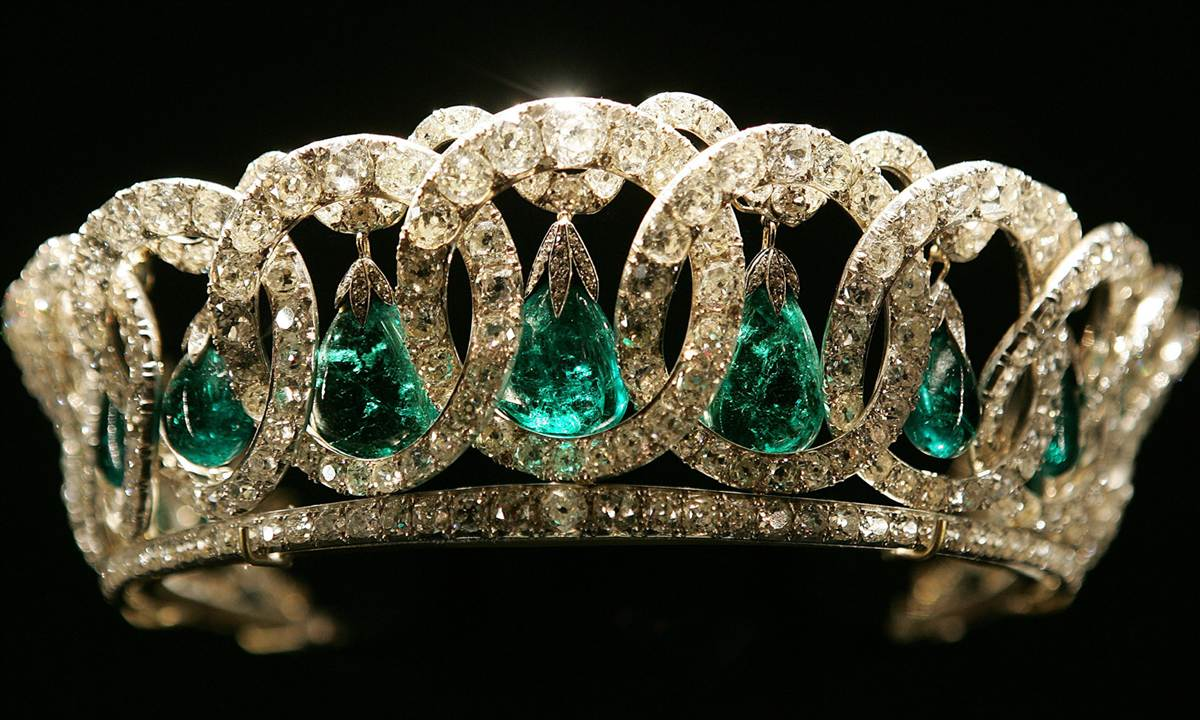
\includegraphics[width=2in]{crown.jpg}
\end{figure}  
} 



\end{enumerate}

\problem{We've now proven the CLT, but you may not viscerally feel it yet since all you did is just a bunch of math in bilateral Laplace transform space (which doesn't exactly exalt the spirit). This problem is here to make you really understand the power of this technology. This is a preview to confidence intervals and hypothesis testing which will be the topics of the remainder of this course.}

\begin{enumerate}
\easysubproblem{Image $X \sim \bernoulli{\half}$. Run the following code in \texttt{R} and print out (in black and white) the result of the following. Does this look like the PMF of $X$? }

\begin{verbatim}
#first line placeholder
par(mfrow = c(1, 1))
N = 10000
xs = rbinom(N, 1, 0.5)
h = hist(xs, breaks = 100, plot = FALSE)
h$counts = h$counts / sum(h$counts)
plot(h)
#last line placeholder
\end{verbatim}


\easysubproblem{Now we're going to imagine $X_1, \ldots, X_n \iid \bernoulli{p = 0.5}$ and compute our friend:

\beqn
C_n = \sqrt{n} \Zbar = \frac{\Xbar - \mu}{\frac{\sigma}{\sqrt{n}}}
\eeqn

Since we know $\mu = p = 0.5$ and $\sigma = \sqrt{p(1-p)} = \sqrt{0.5 (1 - 0.5)} = 0.5$,

\beqn
C_n =  \frac{\Xbar - 0.5}{\frac{0.5}{\sqrt{n}}}
\eeqn

We are going to look at the distribution of $C_n$ for different values of $n$. Remember $C = \limitn C_n$ should be distributed as $\stdnormnot$. Run the following code in \texttt{R} and print out (in black and white) the result (please be patient):

This will look at the estimated PDF for $C_n$ for $n = 10, 100, 1000, 5000, 10000, 50000$. At what $n$ value does it appear that $C_n$ converged to a $\stdnormnot$? Pay attention to gaps of whitespace in these plots. They mean there's no support there! The standard normal has support everywhere. If it never converges, write \qu{never.} }

\begin{verbatim}
#first line placeholder
par(mfrow = c(3, 2))
N = 10000
mu = 0.5
sigma = 0.5
for (n in c(10, 100, 1000, 5000, 10000, 50000)){
  xs = matrix(rbinom(n * N, 1, mu), ncol = N)
  xbars = (colMeans(xs) - mu) / (sigma / sqrt(n))
  hist(xbars, breaks = 100, xlim = c(-4, 4), 
    main = paste("PDF estimate of Cn for n =", n), col = "blue")
}
#last line placeholder
\end{verbatim}~\spc{1}

\easysubproblem{Now we're going to imagine $X_1, \ldots, X_n \iid \bernoulli{p = 0.1}$ which is more skewed towards failures. Since we know $\mu = p = 0.1$ and $\sigma = \sqrt{p(1-p)} = \sqrt{0.1 (1 - 0.1)} = 0.3$,

\beqn
C_n =  \frac{\Xbar - 0.1}{\frac{0.3}{\sqrt{n}}}
\eeqn

We are going to look at the distribution of $C_n$ for different values of $n$. Remember $C = \limitn C_n$ should be distributed as $\stdnormnot$. Run the following code in \texttt{R} and print out (in black and white) the result (please be patient).

This will look at the estimated PDF for $C_n$ for $n = 10, 100, 1000, 5000, 10000, 50000$. At what $n$ value does it appear that $C_n$ converged to a $\stdnormnot$? Pay attention to gaps of whitespace in these plots. They mean there's no support there! The standard normal has support everywhere. If it never converges, write \qu{never.} }

\begin{verbatim}
#first line placeholder
par(mfrow = c(3, 2))
N = 10000
mu = 0.1
sigma = 0.3
for (n in c(10, 100, 1000, 5000, 10000, 50000)){
  xs = matrix(rbinom(n * N, 1, mu), ncol = N)
  xbars = (colMeans(xs) - mu) / (sigma / sqrt(n))
  hist(xbars, breaks = 100, xlim = c(-4, 4), 
    main = paste("PDF estimate of Cn for n =", n), col = "blue")
}
#last line placeholder
\end{verbatim}
~\spc{2}


\easysubproblem{Now we're going to imagine $X_1, \ldots, X_n \iid \binomial{n = 100}{p = 0.5}$. Since we know $\mu = np = 50$ and $\sigma = \sqrt{np(1-p)} = \sqrt{100 (0.5) (1 - 0.5)} = 5$,

\beqn
C_n =  \frac{\Xbar - 50}{\frac{5}{\sqrt{n}}}
\eeqn

We are going to look at the distribution of $C_n$ for different values of $n$. Remember $C = \limitn C_n$ should be distributed as $\stdnormnot$. Run the following code in \texttt{R} and print out (in black and white) the result (please be patient).

This will look at the estimated PDF for $C_n$ for $n = 10, 100, 1000, 5000$. At what $n$ value does it appear that $C_n$ converged to a $\stdnormnot$? Pay attention to gaps of whitespace in these plots. They mean there's no support there! The standard normal has support everywhere. If it never converges, write \qu{never.} \\ }

\begin{verbatim}
#first line placeholder
par(mfrow = c(2, 2))
N = 10000
mu = 50
sigma = 5
for (n in c(10, 100, 1000, 5000)){
  xs = matrix(rbinom(n * N, 100, 0.5), ncol = N)
  xbars = (colMeans(xs) - mu) / (sigma / sqrt(n))
  hist(xbars, breaks = 100, xlim = c(-4, 4), 
    main = paste("PDF estimate of Cn for n =", n), col = "blue")
}
#last line placeholder
\end{verbatim}~\spc{5}

\easysubproblem{Now we're going to imagine $X_1, \ldots, X_n \iid \poisson{\lambda = 7}$. Since we know $\mu = \lambda = 7$ and $\sigma = \sqrt{\lambda} = \sqrt{7} = 2.6458$,

\beqn
C_n =  \frac{\Xbar - 7}{\frac{2.6458}{\sqrt{n}}}
\eeqn

We are going to look at the distribution of $C_n$ for different values of $n$. Remember $C = \limitn C_n$ should be distributed as $\stdnormnot$. Run the following code in \texttt{R} and print out (in black and white) the result (please be patient).

This will look at the estimated PDF for $C_n$ for $n = 10, 100, 1000, 5000, 10000, 50000$. At what $n$ value does it appear that $C_n$ converged to a $\stdnormnot$? Pay attention to gaps of whitespace in these plots. They mean there's no support there! The standard normal has support everywhere. If it never converges, write \qu{never.} } \pagebreak

\begin{verbatim}
#first line placeholder
par(mfrow = c(3, 2))
N = 10000
mu = 7
sigma = 2.6458
for (n in c(10, 100, 1000, 5000, 10000, 50000)){
  xs = matrix(rpois(n * N, mu), ncol = N)
  xbars = (colMeans(xs) - mu) / (sigma / sqrt(n))
  hist(xbars, breaks = 100, xlim = c(-4, 4), 
    main = paste("PDF estimate of Cn for n =", n), col = "blue")
}
#last line placeholder
\end{verbatim}~\spc{1}


\easysubproblem{Now we're going to imagine $X_1, \ldots, X_n \iid \exponential{\lambda = 7}$. Since we know $\mu = 1 / \lambda = 0.1429$ and $\sigma = 1 / \lambda =  0.1429$,

\beqn
C_n =  \frac{\Xbar - 0.1429}{\frac{0.1429}{\sqrt{n}}}
\eeqn

We are going to look at the distribution of $C_n$ for different values of $n$. Remember $C = \limitn C_n$ should be distributed as $\stdnormnot$. Run the following code in \texttt{R} and print out (in black and white) the result (please be patient).

This will look at the estimated PDF for $C_n$ for $n = 10, 100, 1000, 5000$. At what $n$ value does it appear that $C_n$ converged to a $\stdnormnot$? Pay attention to gaps of whitespace in these plots. They mean there's no support there! The standard normal has support everywhere. If it never converges, write \qu{never.} }

\begin{verbatim}
#first line placeholder
par(mfrow = c(2, 2))
N = 10000
mu = 0.1429
sigma = 0.1429
for (n in c(10, 100, 1000, 5000)){
  xs = matrix(rexp(n * N, 7), ncol = N)
  xbars = (colMeans(xs) - mu) / (sigma / sqrt(n))
  hist(xbars, breaks = 100, xlim = c(-4, 4), 
    main = paste("PDF estimate of Cn for n =", n), col = "blue")
}
#last line placeholder
\end{verbatim}

\easysubproblem{Now we're going to imagine $X_1, \ldots, X_n \iid \normnot{\mu = 3}{\sigsq = 6^2}$. Since we know $\mu = 3$ and $\sigma = 6$,

\beqn
C_n =  \frac{\Xbar - 3}{\frac{6}{\sqrt{n}}}
\eeqn

We are going to look at the distribution of $C_n$ for different values of $n$. Remember $C = \limitn C_n$ should be distributed as $\stdnormnot$. Run the following code in \texttt{R} and print out (in black and white) the result (please be patient).

This will look at the estimated PDF for $C_n$ for $n = 10, 100, 1000, 5000$. At what $n$ value does it appear that $C_n$ converged to a $\stdnormnot$? Pay attention to gaps of whitespace in these plots. They mean there's no support there! The standard normal has support everywhere. If it never converges, write \qu{never.} }

\begin{verbatim}
#first line placeholder
par(mfrow = c(2, 2))
N = 10000
mu = 3
sigma = 6
for (n in c(10, 100, 1000, 5000)){
  xs = matrix(rnorm(n * N, 3, 6), ncol = N)
  xbars = (colMeans(xs) - mu) / (sigma / sqrt(n))
  hist(xbars, breaks = 100, xlim = c(-4, 4), 
    main = paste("PDF estimate of Cn for n =", n), col = "blue")
}
#last line placeholder
\end{verbatim}~\spc{1}

\intermediatesubproblem{Why did this converge immediately? See question 2(m) for the answer. }\spc{2}

\easysubproblem{Now we're going to get more elaborate. Imagine the following PDF: 

I will consider this to be called the \qu{bathtub function.} This is not a real brand name distribution. I just made it up and it won't be on the test. Write about why you think I called it the \qu{bathtub function.} Does this look like a bell curve at all?? }

\begin{verbatim}
#first line placeholder
par(mfrow = c(1, 1))
N = 10000
xs = 100 * rbeta(N, 0.1, 0.1)
h = hist(xs, breaks = 1000, plot = FALSE)
h$counts = h$counts / sum(h$counts)
plot(h)
#last line placeholder
\end{verbatim}~\spc{2}

\easysubproblem{Now we're going to make sure the central limit theorem works even with stuff that's as crazy as the bathtub. Imagine $X_1, \ldots, X_n \iid \text{bathtub}$. By advanced math, I know $\mu = 50$ and $\sigma = 45.6436$ thus,

\beqn
C_n =  \frac{\Xbar - 50}{\frac{45.6436}{\sqrt{n}}}
\eeqn

We are going to look at the distribution of $C_n$ for different values of $n$. Remember $C = \limitn C_n$ should be distributed as $\stdnormnot$. Run the following code in \texttt{R} and print out (in black and white) the result (please be patient).

This will look at the estimated PDF for $C_n$ for $n = 2, 5, 10, 50, 100, 1000$. At what $n$ value does it appear that $C_n$ converged to a $\stdnormnot$? Pay attention to gaps of whitespace in these plots. They mean there's no support there! The standard normal has support everywhere. If it never converges, write \qu{never.} }

\begin{verbatim}
#first line placeholder
par(mfrow = c(3, 2))
N = 10000
mu = 50
sigma = 45.6436
for (n in c(2, 5, 10, 50, 100, 1000)){
  xs = matrix(100 * rbeta(n * N, 0.1, 0.1), ncol = N)
  xbars = (colMeans(xs) - mu) / (sigma / sqrt(n))
  hist(xbars, breaks = 100, xlim = c(-4, 4), 
    main = paste("PDF estimate of Cn for n =", n), col = "blue")
}
#last line placeholder
\end{verbatim}

\easysubproblem{Let's sum up what we've learned in this problem. The central limit states as $n \rightarrow \infty$ (i.e. it gets big) then $C_n$ becomes a standard normal. Does it become a standard normal at different rates depending on the distribution of the r.v. being sampled? Yes/no is fine.} \spc{2}

\end{enumerate}

\problem{Now that we've now proven the CLT, we are going to use it a little bit. Assume $X_1, \ldots, X_n \iid$ something with mean $\mu$ and standard error $\sigma$.}

\begin{enumerate}

\easysubproblem{Assume $n$ is large enough for the CLT to kick in, show that:

\beqn
\Xbar \sim \normnot{\mu}{\squared{\frac{\sigma}{\sqrt{n}}}}
\eeqn }\spc{1.5}

\easysubproblem{Assume $n$ is large enough for the CLT to kick in, show that:

\beqn
T_n \sim \normnot{n\mu}{\squared{\sqrt{n}\sigma}}
\eeqn }\spc{1.5}


\easysubproblem{Let $X_1, \ldots, X_n \iid \bernoulli{p}$ and let $\Phat := \Xbar$. Assume $n$ is large enough for the CLT to kick in, show that:

\beqn
\Phat \sim \normnot{p}{\squared{\sqrt{\frac{p(1-p))}{n}}}}
\eeqn }\spc{1.5}

\end{enumerate}
\end{document}

